% !TeX root = RJwrapper.tex
\title{Environmental fluoxetine promotes skin cell proliferation and
wound healing}
\author{by Roa Hanoun and Jero Eyras}

\maketitle

\abstract{%
Pharmaceutical pollutants, including the antidepressant fluoxetine (FLX,
commercial name: Prozac), are increasingly detected in aquatic
environments, raising concerns about their effects on non-target
organisms, including humans. The original study demonstrated that
environmentally-relevant FLX concentrations promote wound closure in
human skin biopsies and keratinocytes through enhanced cell
proliferation and serotonin signalling, supported by transcriptomic,
phosphoproteomic, and kinase profiling analyses. Building on these
findings, the present study extends the transcriptomic analysis by
examining gene expression in scratched HaCaT keratinocytes exposed to
540 ng/L FLX at two time points: 6 and 36 hours. Differentially
expressed genes (DEGs) were identified at each time point and compared
to unexposed control cells, with an intersection analysis performed
between both conditions. We identified 147 DEGs at 6 hours and 250 DEGs
at 36 hours, with upregulated genes associated with cell proliferation
and cellular stress defence mechanisms. The difference in DEG numbers
compared to the original study reflects sample quality filtering applied
during data processing. These results provide a more detailed temporal
resolution of FLX-induced transcriptomic changes and support the
conclusion that environmental FLX exposure modulates gene expression in
ways that may meaningfully impact skin wound healing.
}

\section{Introduction}\label{introduction}

Pharmaceutical pollution has become a growing environmental concern,
particularly the presence of antidepressants in aquatic ecosystems.
Fluoxetine (FLX), commercially known as Prozac, is one of the most
widely prescribed selective serotonin reuptake inhibitors (SSRIs) and
works by blocking the reabsorption of serotonin in the brain, thereby
increasing serotonin availability and improving mood regulation. Due to
incomplete metabolisation in the human body and inadequate removal by
wastewater treatment plants, FLX is consistently detected in surface
waters at concentrations ranging from nanograms to micrograms per liter.

Serotonin is not only a neurotransmitter but also plays a
well-established role in peripheral tissues, including the skin, where
it is involved in regulating cell proliferation and wound healing. Wound
healing is a complex and tightly coordinated biological process that
proceeds through three overlapping phases: inflammation, proliferation,
and tissue remodeling. During the proliferation phase, keratinocytes ---
the dominant cell type of the outermost skin layer (the epidermis) ---
migrate toward the wound edge and actively divide to restore the skin
barrier. Any disruption or enhancement of this process can have
significant clinical implications. Given that FLX modulates serotonin
signalling, and serotonin itself plays a role in keratinocyte activity,
it is biologically plausible that environmental FLX exposure could
meaningfully influence skin repair mechanisms.

The original study by \citep{rodriguez:2024} was the first to
investigate this link experimentally, using a multi-omics approach
combining transcriptomics, phosphoproteomics, and kinase profiling.
Their transcriptomic analysis identified 350 differentially expressed
genes (DEGs) in FLX-exposed keratinocytes, with upregulated genes linked
to cell proliferation and tissue morphogenesis, and downregulated genes
associated with mitochondrial function and metabolism
\citep{rodriguez:2024}. These findings provided a molecular basis for
the observed enhancement in wound closure, but left room for deeper
temporal investigation of how gene expression changes evolve over time
during FLX exposure.

Transcriptomics is the large-scale study of all RNA molecules expressed
in a cell or tissue at a given moment, essentially providing a snapshot
of which genes are active and to what degree. By comparing gene
expression between exposed and unexposed cells, it is possible to
identify which biological processes are being switched on or off in
response to a treatment. In this study, we use RNA sequencing (RNA-seq)
data analysed with DESeq2, a statistical tool specifically designed to
detect differentially expressed genes from count-based sequencing data
while accounting for biological variability between samples.

The present study focuses exclusively on the transcriptomic component of
the original research. We analysed gene expression in scratched HaCaT
human keratinocytes exposed to 540 ng/L FLX at two time points: 6 and 36
hours, mirroring the time points used in the transcriptomic section of
the original study \citep{rodriguez:2024}. The 6-hour time point
captures the early transcriptional response to FLX exposure, reflecting
immediate cellular adjustments, while the 36-hour time point represents
a later stage where more sustained gene expression changes associated
with active wound closure are expected. Our central research question
is: does FLX exposure significantly alter gene expression in human
keratinocytes in ways that support enhanced wound healing, and how does
this response evolve between 6 and 36 hours of exposure? To address
this, DEGs were identified at each time point and compared to unexposed
control cells, followed by enrichment analysis to map these genes to
relevant biological pathways. An intersection analysis was further
performed to identify genes consistently differentially expressed across
both time points. We also explored whether enrichment analysis could
reveal additional gene functions and pathways beyond those reported in
the original article \citep{rodriguez:2024}.

\section{Materials and Methods}\label{materials-and-methods}

\subsection{Cells and clinical
samples}\label{cells-and-clinical-samples}

HaCaT cells are immortalised human keratinocytes derived from normal
adult human skin and were obtained from AddexBio. Due to their
well-characterised behaviour and relevance to skin biology, HaCaT cells
are widely established as a model system in dermatological research.
Cells were maintained in 5\% CO2 incubation chambers at 37 °C and
subcultured every 3 days or upon reaching approximately 80\% confluency.

To investigate the transcriptomic effects of Fluoxetine (FLX) on wound
healing, a scratch assay was performed on HaCaT cell monolayers.
Following the scratch, cells were treated with FLX at a concentration of
540 ng/L. Conditions were defined as a combination of treatment (FLX
vs.~control) and time post-scratch (6 h and 36 h), resulting in a total
of four samples across both conditions.

\subsection{RNA sequencing}\label{rna-sequencing}

HaCaT cells were scratched three times per well in 6-well plates, and
total RNA was isolated at 6 h and 36 h post-scratch using the PureLink™
RNA Mini Kit (Thermo Fisher Scientific), following the manufacturer's
instructions. Library preparation and RNA sequencing were carried out by
Novogene Co.~Ltd.~(Cambridge, UK) using the Illumina NovaSeq 6000
platform. The sequencing output consisted of two files, one for each
comparison (6 h and 36 h), each containing one FLX-exposed sample and
one untreated control sample. Each file included gene annotation columns
(gene name, gene ID, chromosome, start and end positions, strand,
length, and biotype), raw read counts per sample, FPKM-normalised
expression values, and statistical outputs including log2. fold change,
p-value, and adjusted p-value (padj). Raw read counts were used as input
for all downstream differential expression analysis.

\subsection{Data Pre-processing}\label{data-pre-processing}

Prior to differential expression analysis, sample quality was assessed
using multiple visualizations. Raw count data were normalized using
Variance Stabilizing Transformation (VST) as implemented in
\texttt{DESeq2}, and Poisson distance-based normalization was applied to
measure dissimilarity between samples. Sample-to-sample distances were
visualized using heatmaps and Multidimensional Scaling (MDS) plots,
generated with \texttt{PoiClaClu}, \texttt{ggplot2} and
\texttt{pheatmap} in R, alongside \texttt{DESeq2} built-in plotting
functions. Additionally, bar plots and density plots were produced to
inspect the distribution of counts across samples.

Based on these quality control visualizations, three irregular samples
were identified and removed from the analysis: \texttt{C36-R1} and
\texttt{E36-R3} from the 36-hour dataset, and \texttt{C6-R4} from the
6-hour dataset. Sample removal was performed while ensuring that each
experimental group retained a minimum of three biological replicates, in
order to maintain statistical reliability in the downstream analysis.

\subsection{Differential Expression \& Enrichment
Analysis}\label{differential-expression-enrichment-analysis}

Differential gene expression analysis was performed separately for each
time point (6 h and 36 h) using the DESeq2 R package. Genes were
considered differentially expressed at an unadjusted p-value threshold
of \texttt{p\ \textless{}\ 0.05}. It should be noted that unadjusted
p-values were used in place of adjusted p-values (padj), as this
approach yielded results most comparable to those reported in the
original study.

Entrez gene IDs (ENTREZID) were used as the primary gene identifier for
all enrichment analyses, as they provide a standardised identifier
supported across biological databases. Three complementary enrichment
analyses were performed using the \texttt{clusterProfiler} and
\texttt{ReactomePA} R packages, with gene annotations provided by
\texttt{org.Hs.eg.db}, all applying a significance threshold of pp
\texttt{p\ \textless{}\ 0.05} without p-value adjustment:

\begin{itemize}
\item
  \textbf{Gene Ontology (GO) enrichment (enrichGO)} was performed across
  all three ontology domains --- Biological Process (BP), Cellular
  Component (CC), and Molecular Function (MF) --- as each domain
  captures a distinct and complementary aspect of gene function.
\item
  \textbf{KEGG pathway enrichment (enrichKEGG)} was applied to identify
  which known biological pathways were significantly represented among
  the DEGs, with gene set sizes restricted between 10 and 500 genes.
\item
  \textbf{Reactome pathway enrichment (enrichPathway)} was used to
  identify precise molecular reactions and sub-pathways driven by the
  DEGs.
\end{itemize}

\section{Results}\label{results}

\subsection{DEGs}\label{degs}

No significant differentialy expressed genes where found using a
p-adjusted value \texttt{padj\ \textless{}\ 0.05}. Thus, we proceed with
p-values, although with the warning that we are not using p-adjusted
values. Some significance can be seen in the following p-value
distribution plots for both samples.

\begin{figure}[H]
  \centering
  \begin{subfigure}{0.5\textwidth}
    \includegraphics[width=0.9\linewidth]{images/Pval_6h.png}
    \label{figure:pval_distribution_6h}
  \end{subfigure}%
  \begin{subfigure}{0.5\textwidth}
    \includegraphics[width=0.9\linewidth]{images/Pval_36h.png}
    \label{figure:pval_distribution_36h}
  \end{subfigure}
  \caption{P-value distribution for both sample groups. Namely, distribution shows enough values with significance to proceed with unadjusted p-values.}
  \label{figure:pval_plots}
\end{figure}

With a p-value cutoff of 0.05 we end up with a similar number of DEGs as
the original article. Of course, due to the data cleaning we end up with
a lower amount, while without cleaning it would result in the exact
number. The following volcano plots showcase the resulting DEGs.

\begin{figure}[H]
  \centering
  \begin{subfigure}{0.5\textwidth}
    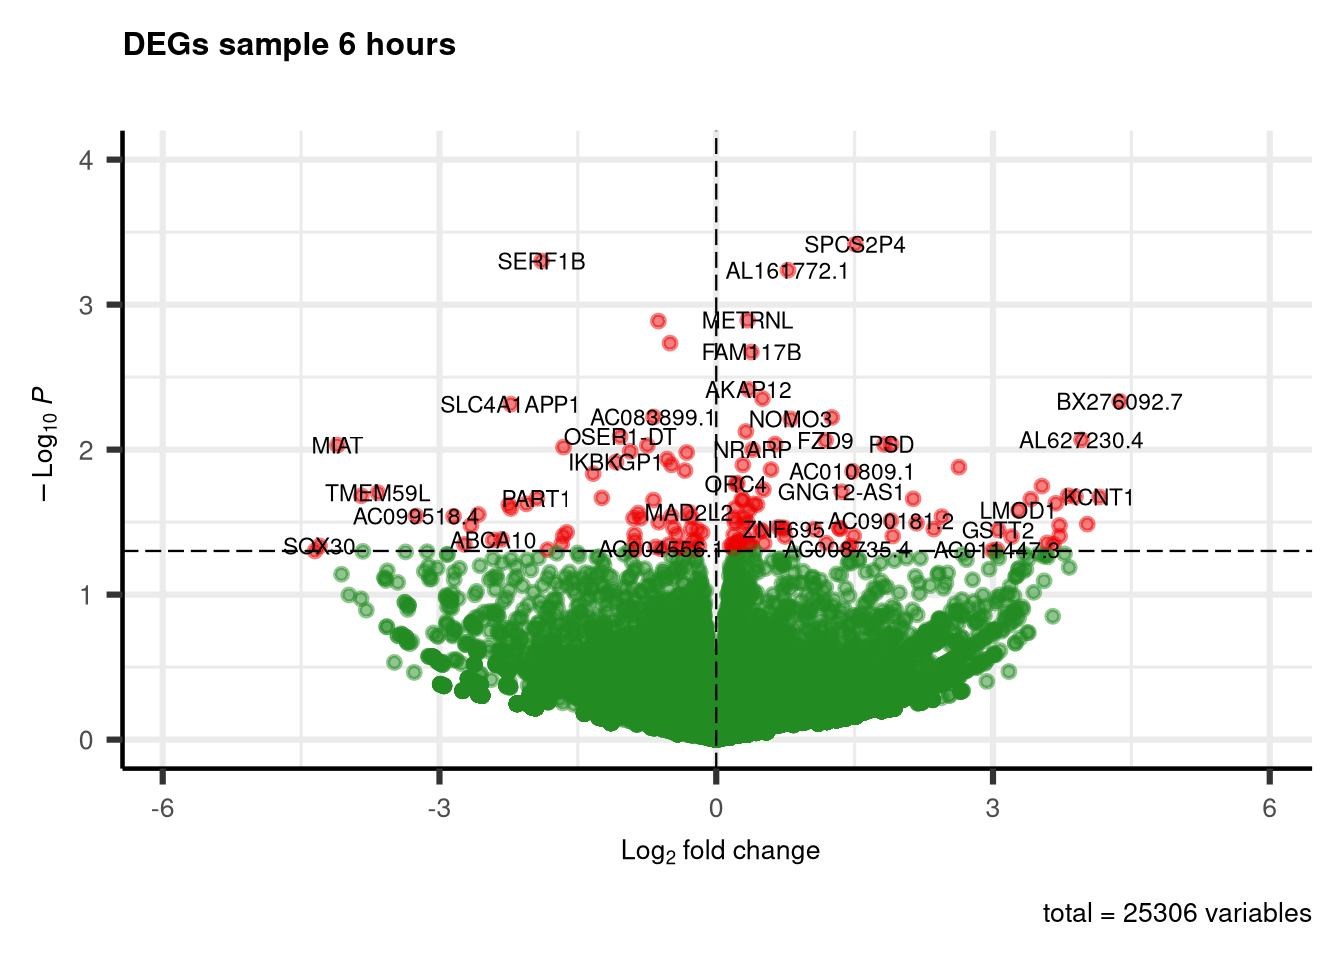
\includegraphics[width=0.9\linewidth]{images/Volcano_6h.png}
    \label{figure:volcano_6h}
  \end{subfigure}%
  \begin{subfigure}{0.5\textwidth}
    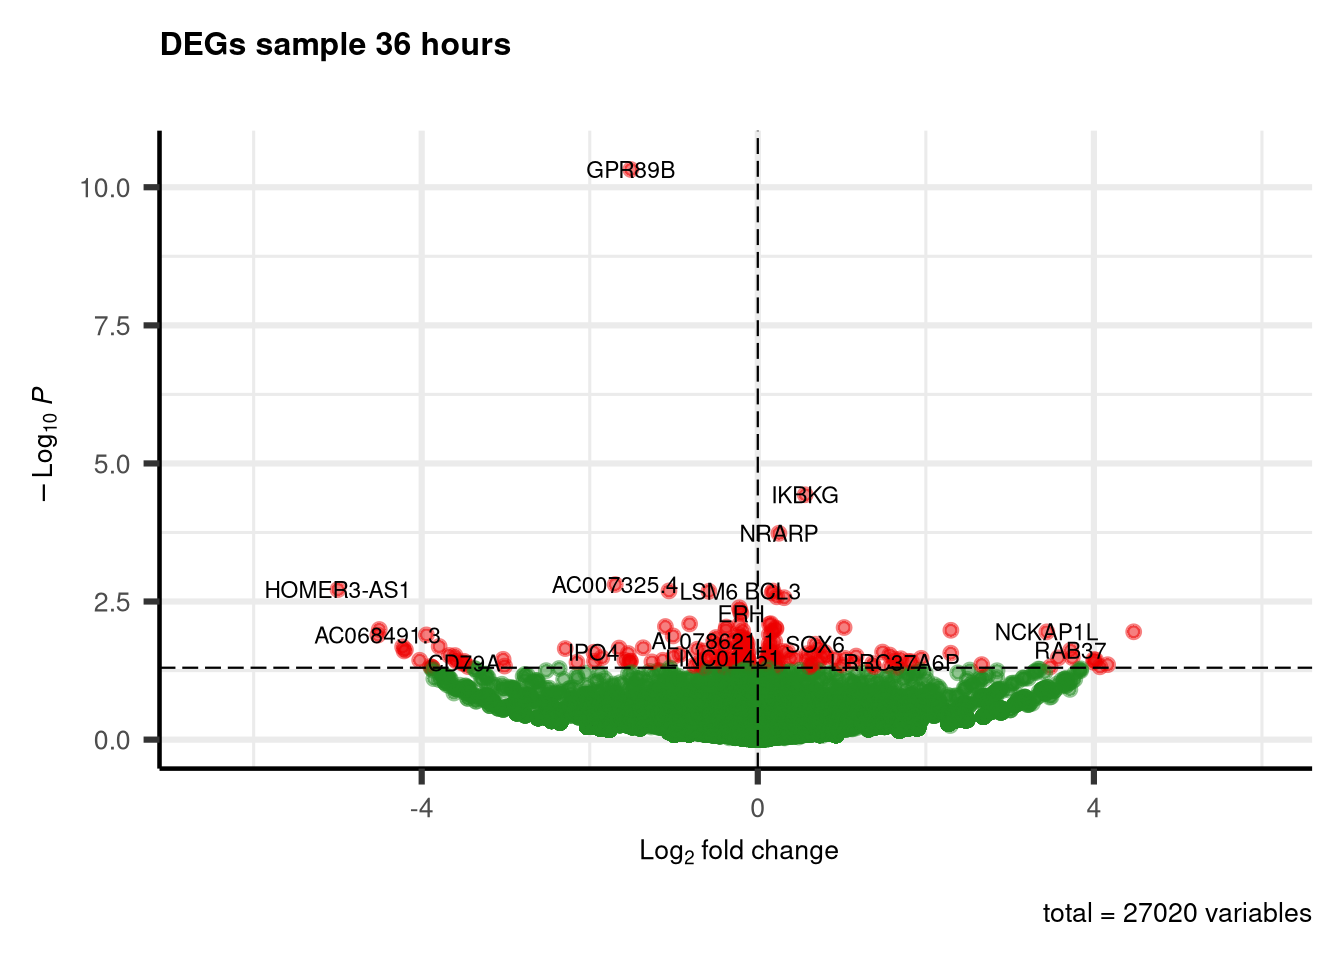
\includegraphics[width=0.9\linewidth]{images/Volcano_36h.png}
    \label{figure:volcano_36h}
  \end{subfigure}
  \caption{Volcano plots for both sample groups. A total of 147 DEGs at +6 hours, 86 upregulated and 61 downregulated, and 242 DEGs at +36 hours, 110 upregulated and 132 downregulated.}
  \label{figure:volcano_plots}
\end{figure}

\subsection{Enrichment Analysis}\label{enrichment-analysis}

\subsubsection{Go Terms}\label{go-terms}

Go enrichment analysis for the +6 hours group shows reduced metabolic
functions in the cell as well as regulation of Wnt signaling, commonly
implicated in regeneration, cancer and epithelial development. For the
+36 hours group upregulated genes are related to cell signaling and
membrane organization.

\begin{figure}[H]
  \centering
  \begin{subfigure}{0.5\textwidth}
    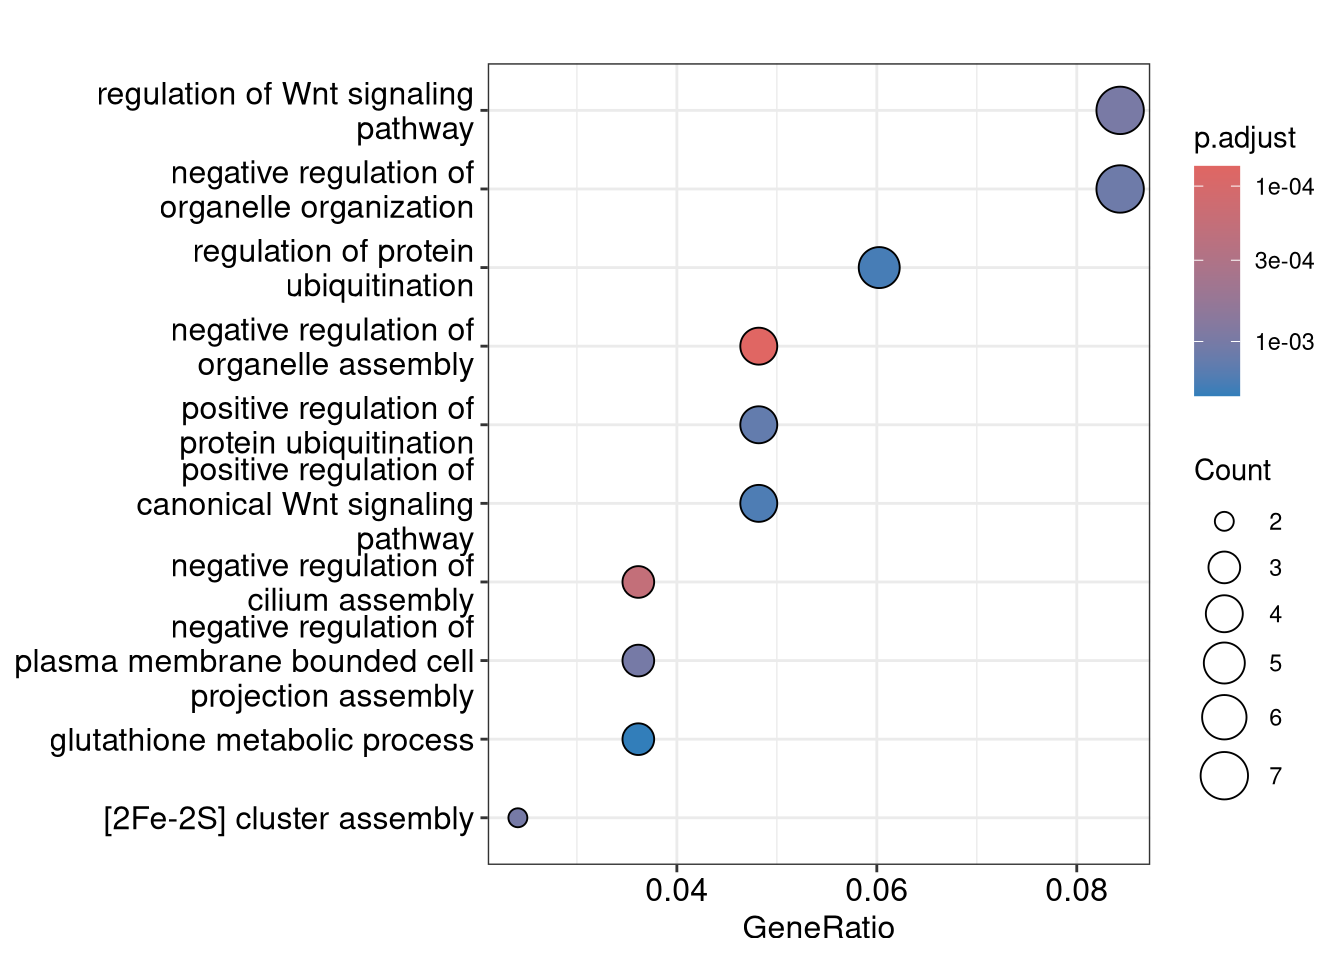
\includegraphics[width=0.9\linewidth]{images/Enrichment_GoBP_6h.png}
    \caption{biological process, +6 hours sample group}
    \label{figure:enrichment_gobp_6h}
  \end{subfigure}%
  \begin{subfigure}{0.5\textwidth}
    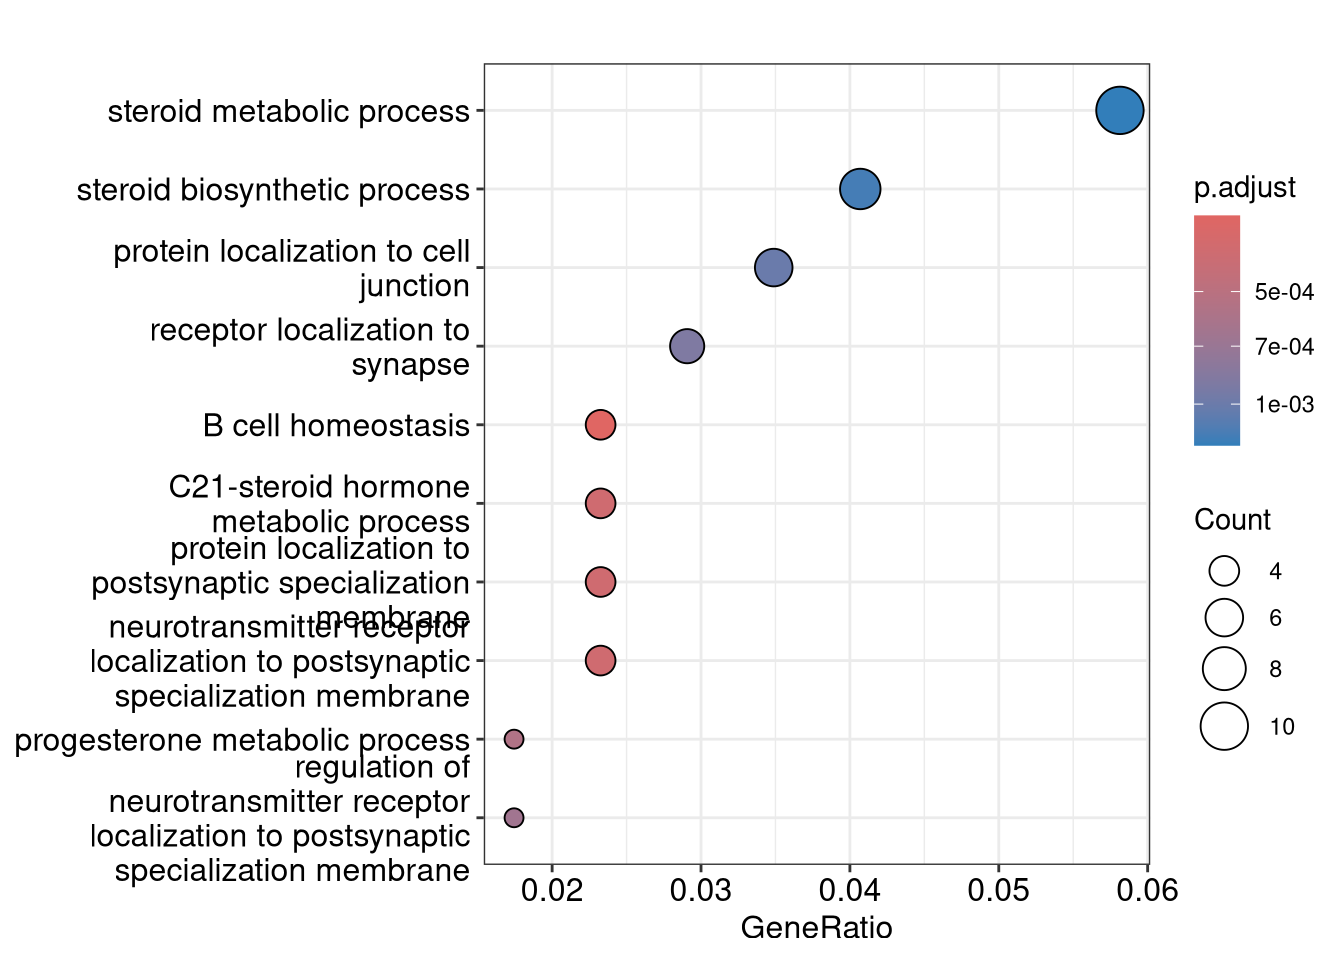
\includegraphics[width=0.9\linewidth]{images/Enrichment_GoBP_36h.png}
    \caption{biological process, +36 hours sample group}
    \label{figure:Enrichment_gobp_36h}
  \end{subfigure}
  \label{figure:enrichment_gobp_plots}
\end{figure}

\begin{figure}[H]
  \centering
  \begin{subfigure}{0.5\textwidth}
    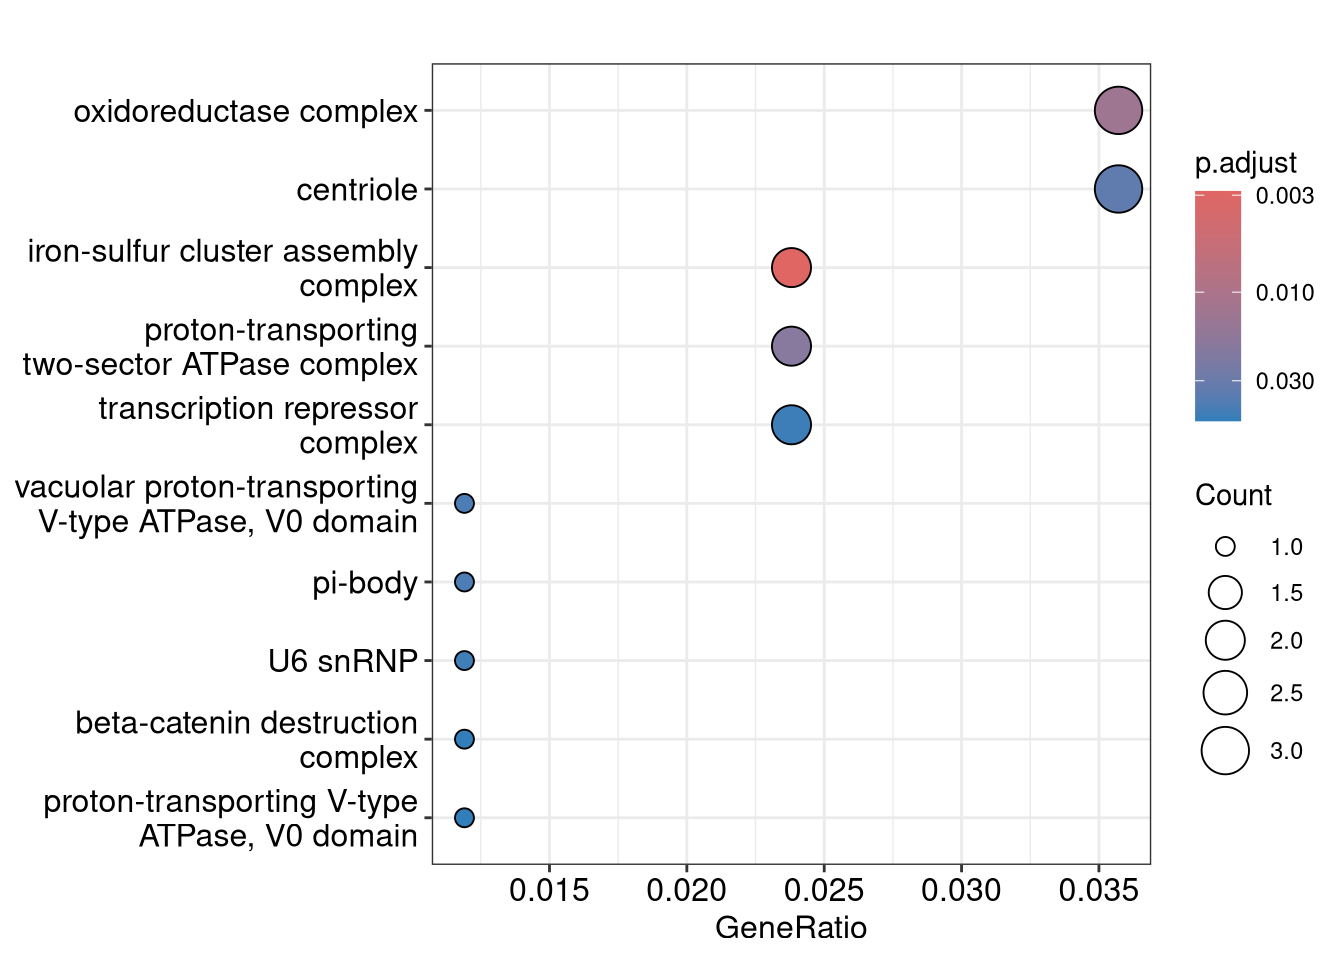
\includegraphics[width=0.9\linewidth]{images/Enrichment_GoCC_6h.png}
    \caption{cellular component, +6 hours sample group}
    \label{figure:enrichment_gocc_6h}
  \end{subfigure}%
  \begin{subfigure}{0.5\textwidth}
    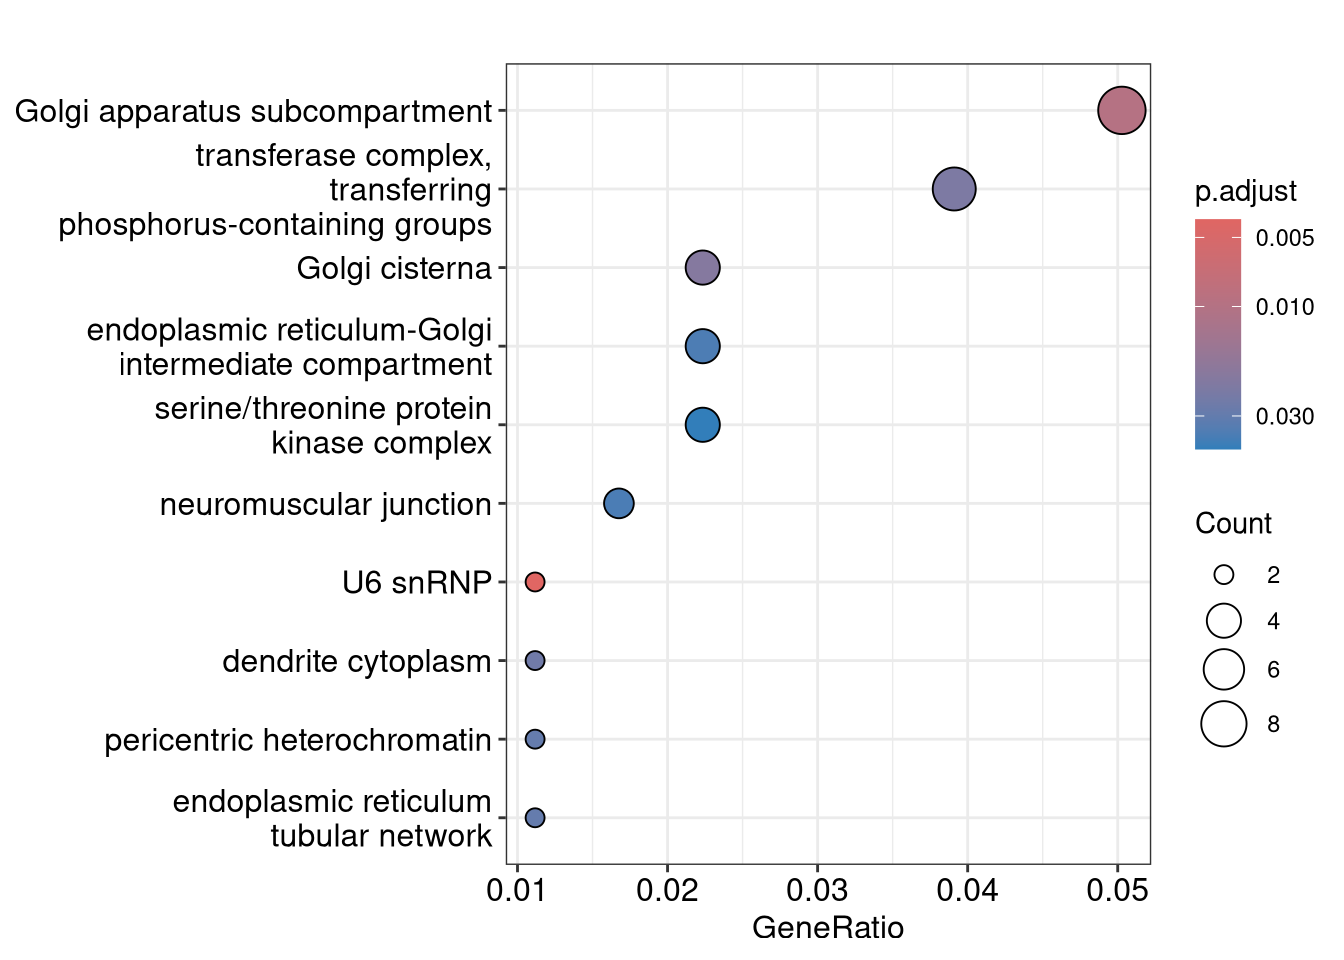
\includegraphics[width=0.9\linewidth]{images/Enrichment_GoCC_36h.png}
    \caption{cellular component, +36 hours sample group}
    \label{figure:Enrichment_gocc_36h}
  \end{subfigure}
  \label{figure:enrichment_gocc_plots}
\end{figure}

\begin{figure}[H]
  \centering
  \begin{subfigure}{0.5\textwidth}
    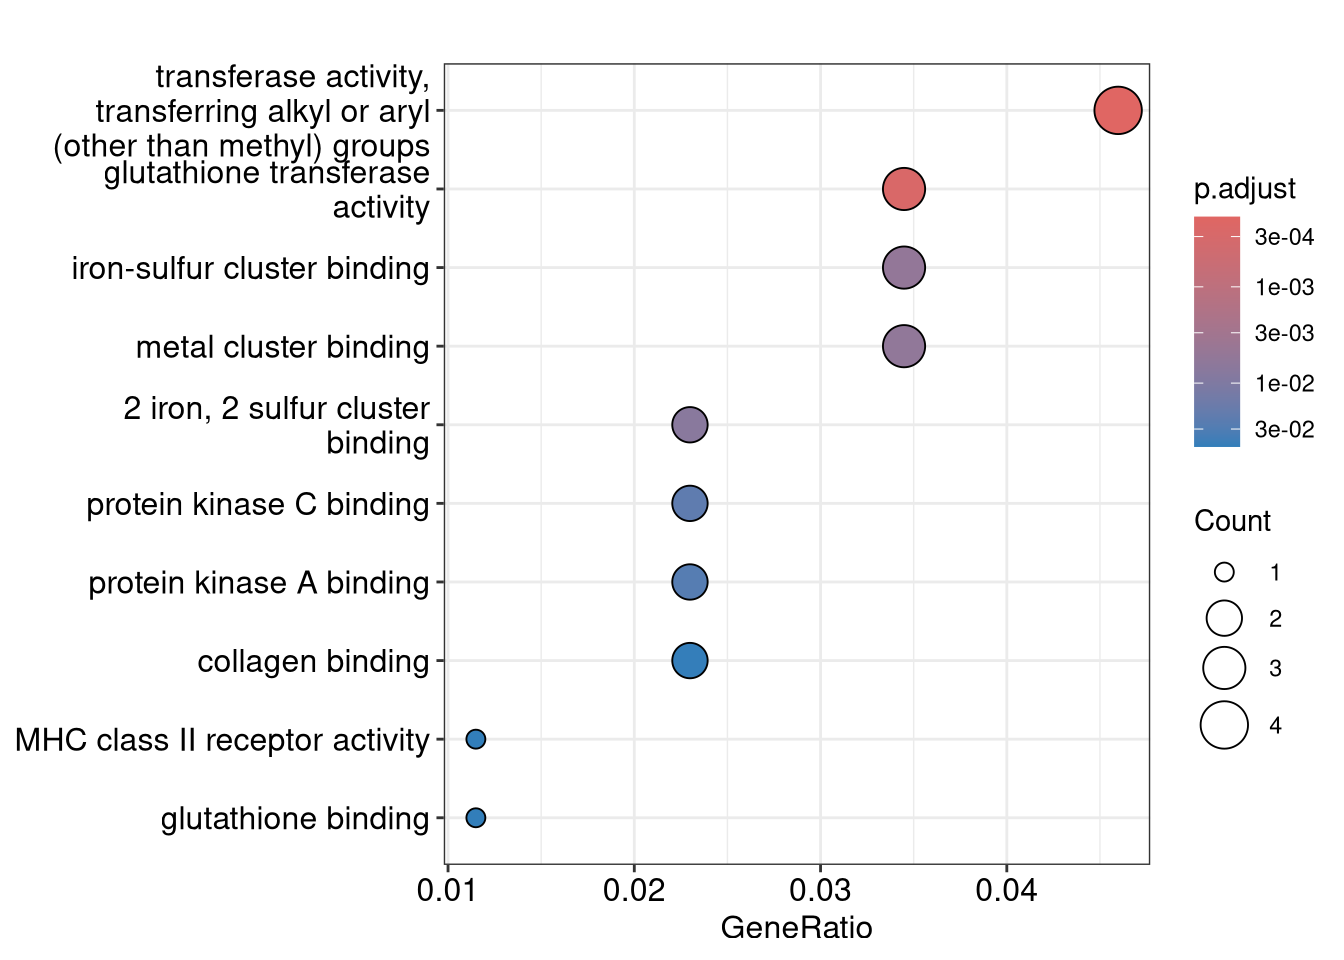
\includegraphics[width=0.9\linewidth]{images/Enrichment_GoMF_6h.png}
    \caption{molecular function, +6 hours sample group}
    \label{figure:enrichment_gomf_6h}
  \end{subfigure}%
  \begin{subfigure}{0.5\textwidth}
    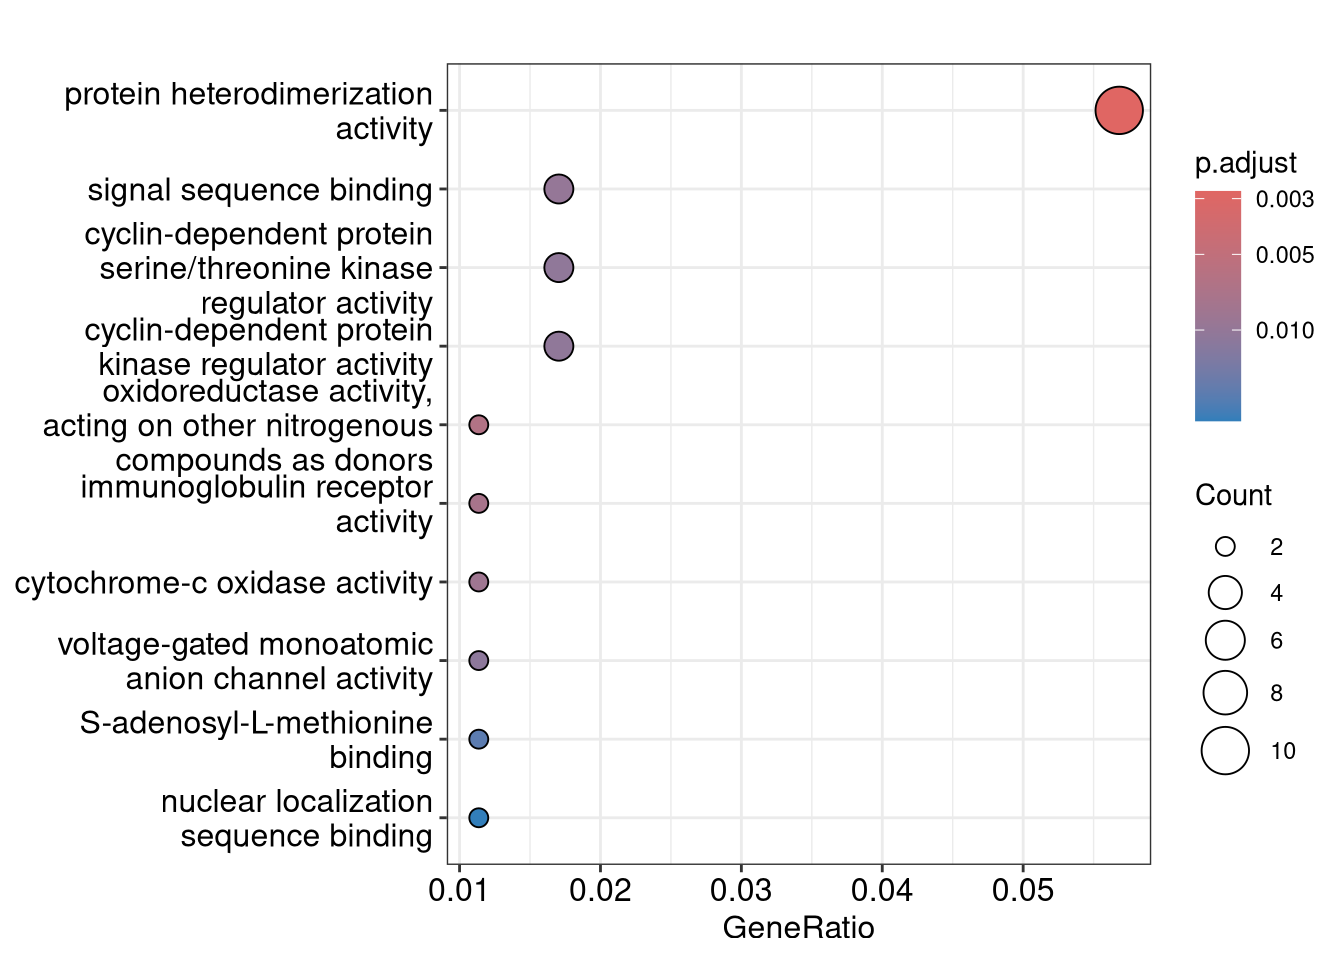
\includegraphics[width=0.9\linewidth]{images/Enrichment_GoMF_36h.png}
    \caption{molecular function, +36 hours sample group}
    \label{figure:Enrichment_gomf_36h}
  \end{subfigure}
  \label{figure:enrichment_gomf_plots}
\end{figure}

\subsubsection{Pathway Analysis}\label{pathway-analysis}

Kegg and reactome analysis results suggest response to oxidative and
chemical stress rather than disease-specific processes for the +6 hours
group, typicaly a detoxification response. Whereas for the +36 hours
group suggests regulation of cellular stress responses, proliferative
signaling, metabolic adaptation, and inflammatory processes.

\begin{figure}[H]
  \centering
  \begin{subfigure}{0.5\textwidth}
    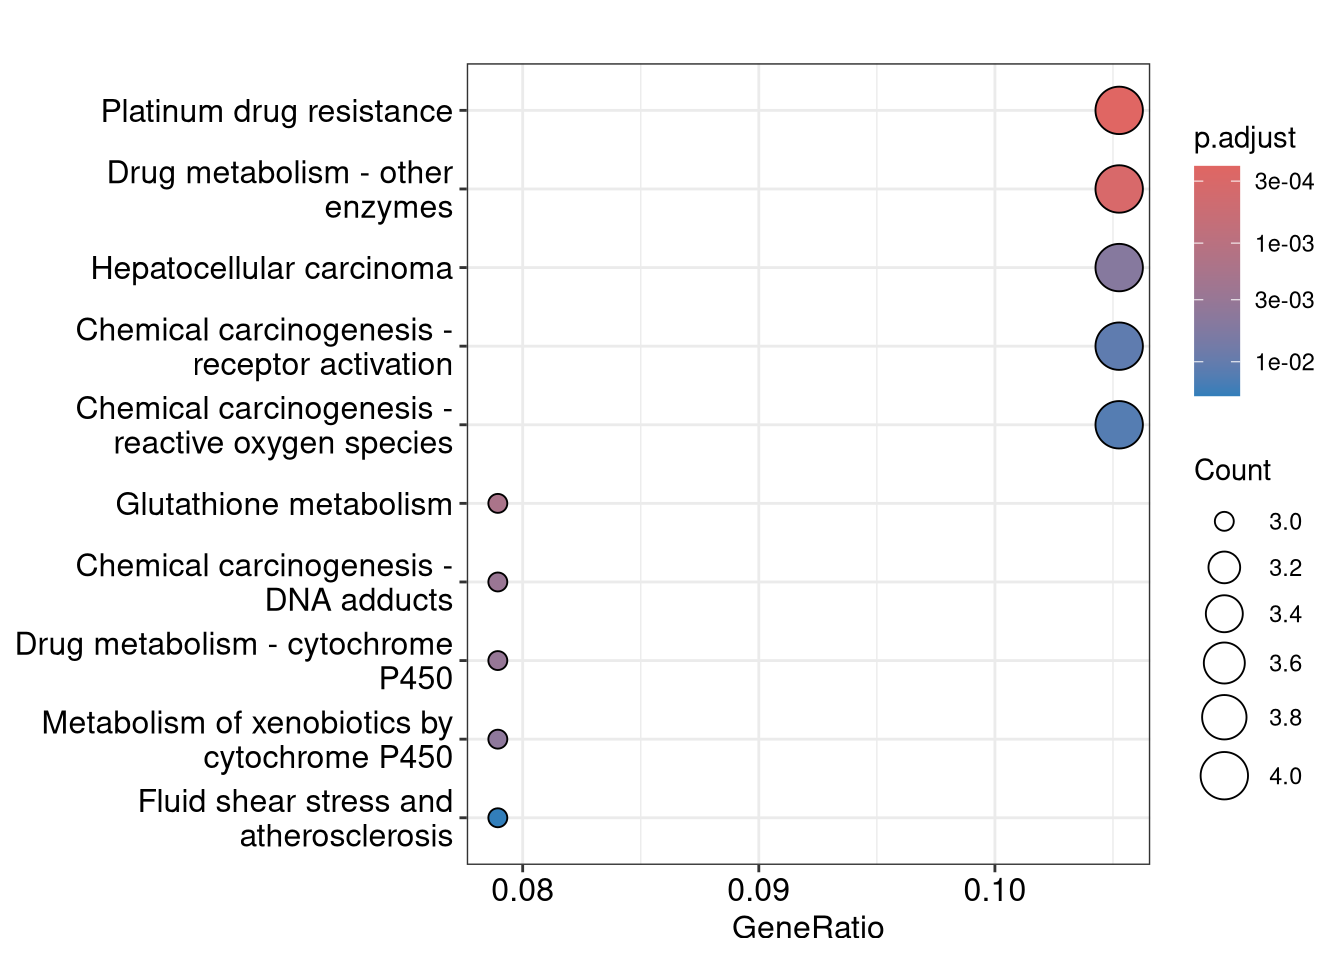
\includegraphics[width=0.9\linewidth]{images/Enrichment_Kegg_6h.png}
    \caption{kegg, +6 hours sample group}
    \label{figure:enrichment_kegg_6h}
  \end{subfigure}%
  \begin{subfigure}{0.5\textwidth}
    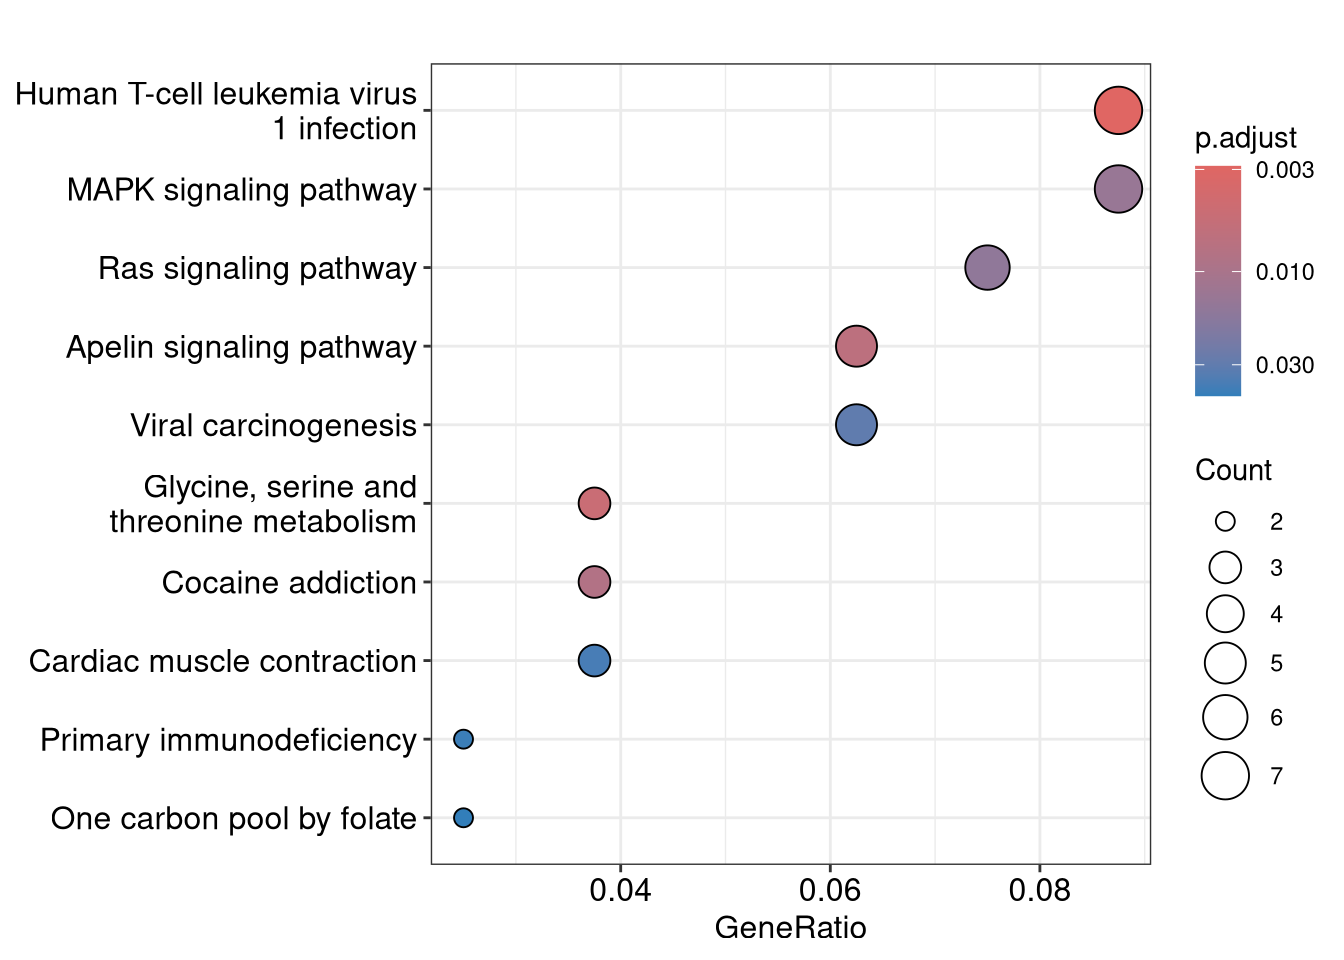
\includegraphics[width=0.9\linewidth]{images/Enrichment_Kegg_36h.png}
    \caption{kegg, +36 hours sample group}
    \label{figure:enrichment_kegg_36h}
  \end{subfigure}
  
  \label{figure:enrichment_kegg_plots}
\end{figure}

\begin{figure}[H]
  \centering
  \begin{subfigure}{0.5\textwidth}
    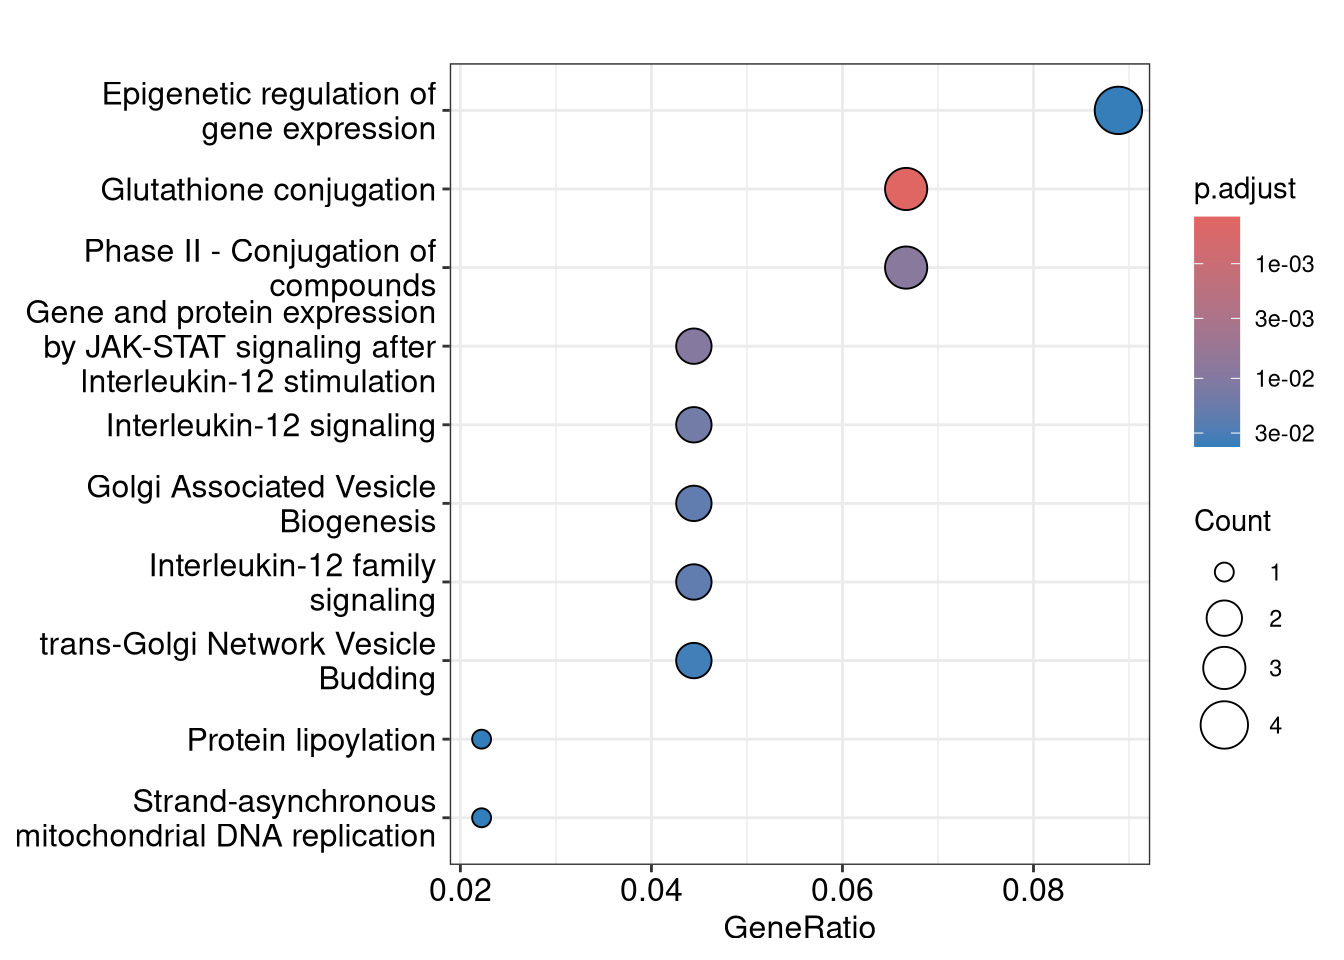
\includegraphics[width=0.9\linewidth]{images/Enrichment_Reactome_6h.png}
    \caption{reactome, +6 hours sample group}
    \label{figure:enrichment_reactome_6h}
  \end{subfigure}%
  \begin{subfigure}{0.5\textwidth}
    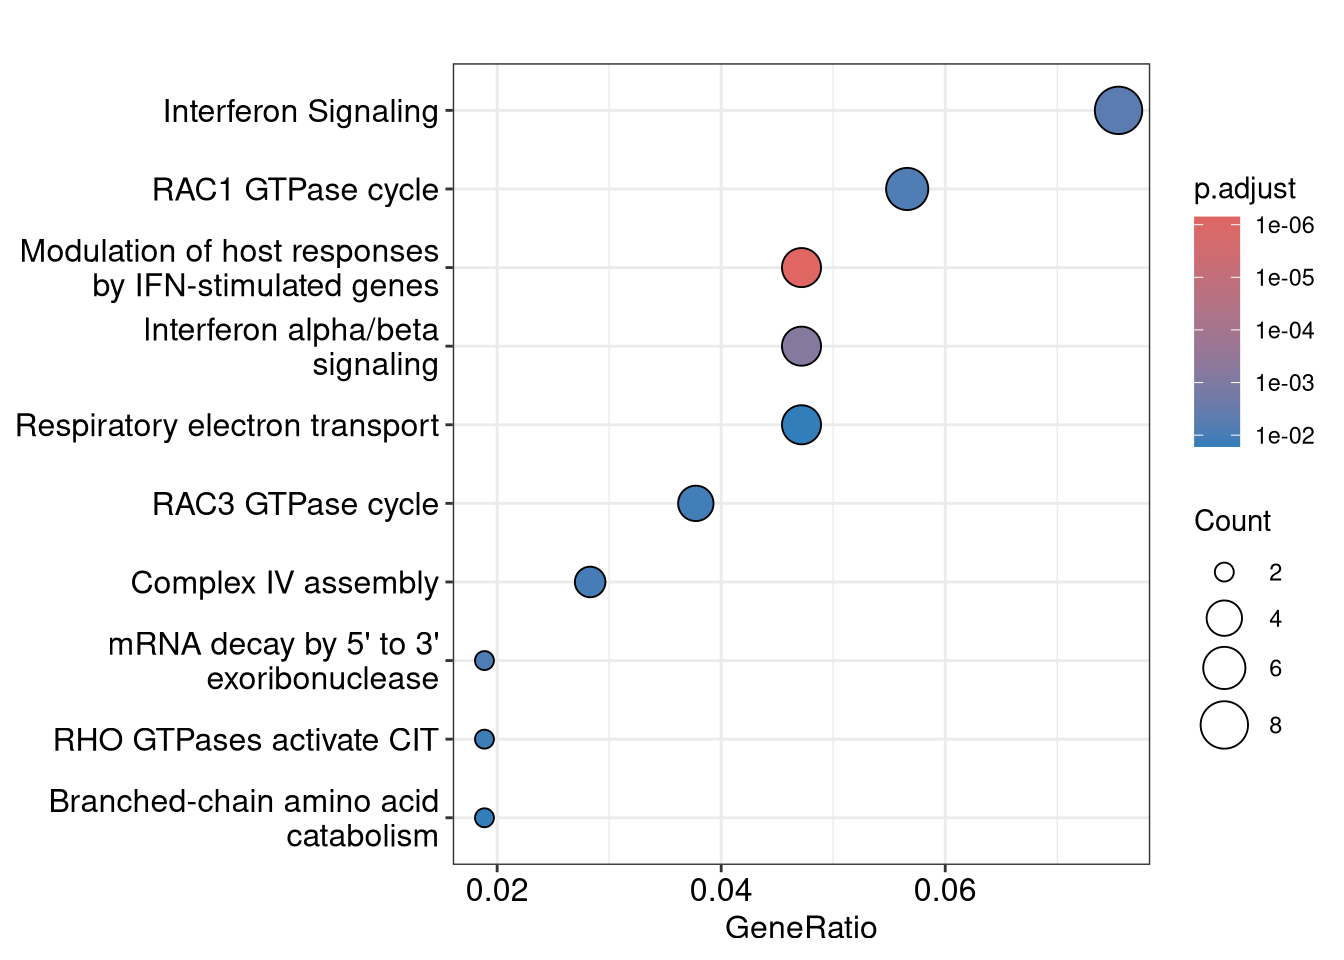
\includegraphics[width=0.9\linewidth]{images/Enrichment_Reactome_36h.png}
    \caption{reactome, +36 hours sample group}
    \label{figure:enrichment_reactome_36h}
  \end{subfigure}
  
  \label{figure:enrichment_reactome_plots}
\end{figure}

\section{Conclusion}\label{conclusion}

Given the results shown above cell signaling and proliferation seem to
be the most notable upsides given the exposure to FLX. Notably, an
initial exposure fires negative responses related to cell stress and
detoxification processes in the cell. There are some week links to
formation of illnesess, specially cancer since we are talking about skin
cells. The most important aspect is that we cannot entirely ensure these
effects given that the p adjusted values proved no significance,
possibly related to sample noise. However, p values showed some
interesting significance which could prompt further research into the
topic.

\section{Discussion}\label{discussion}

The aim of this analysis was to reproduce the differential gene
expression results reported by \citep{rodriguez:2024} using the same
RNA-seq dataset of FLX-exposed HaCaT cells at two time points (6 h and
36 h post-scratch).

\textbf{Comparison with the original article}

Prior to sample cleaning, our DESeq2 analysis yielded exactly the same
number of DEGs as reported in the original article: 165 DEGs at 6 h and
350 DEGs at 36 h. Following the removal of three irregular samples
identified during quality control, the number of DEGs decreased to 147
at 6 h (86 upregulated, 61 downregulated) and 242 at 36 h (110
upregulated, 132 downregulated). The genes identified after cleaning
appear to be a subset of those found before cleaning, suggesting that
sample removal reduced statistical power rather than introducing
different signals.

\textbf{p-value vs adjusted p-value}

Replicating the original DEG counts was only achievable using unadjusted
p-values, despite the article stating padj was used. This discrepancy
remains an open question and a limitation of the current analysis.

\textbf{Overlap between time points}

A Venn diagram comparison revealed three genes shared across both time
points: NRARP, TMEM238, and IKBKGP1. The fact that these three genes
appear in both time points suggests they may play an ongoing role in how
cells respond to FLX during wound healing.

\bibliography{RJreferences}


\address{%
Roa Hanoun\\
Hanze University of Applied Sciences\\%
\\
%
%
%
\href{mailto:rjm.hanoun@st.hanze.nl}{\nolinkurl{rjm.hanoun@st.hanze.nl}}%
}

\address{%
Jero Eyras\\
Hanze University of Applied Sciences\\%
\\
%
%
%
\href{mailto:j.eyras.jimenez@st.hanze.nl}{\nolinkurl{j.eyras.jimenez@st.hanze.nl}}%
}
